\documentclass[border=10pt]{standalone}
\usepackage[svgnames]{xcolor}
\usepackage{amsmath}
\usepackage{pgfplots}
\pgfplotsset{compat=newest}
\usepackage[sfdefault]{FiraSans}
\usepackage{FiraMono}
\renewcommand*\familydefault{\sfdefault}
\begin{document}
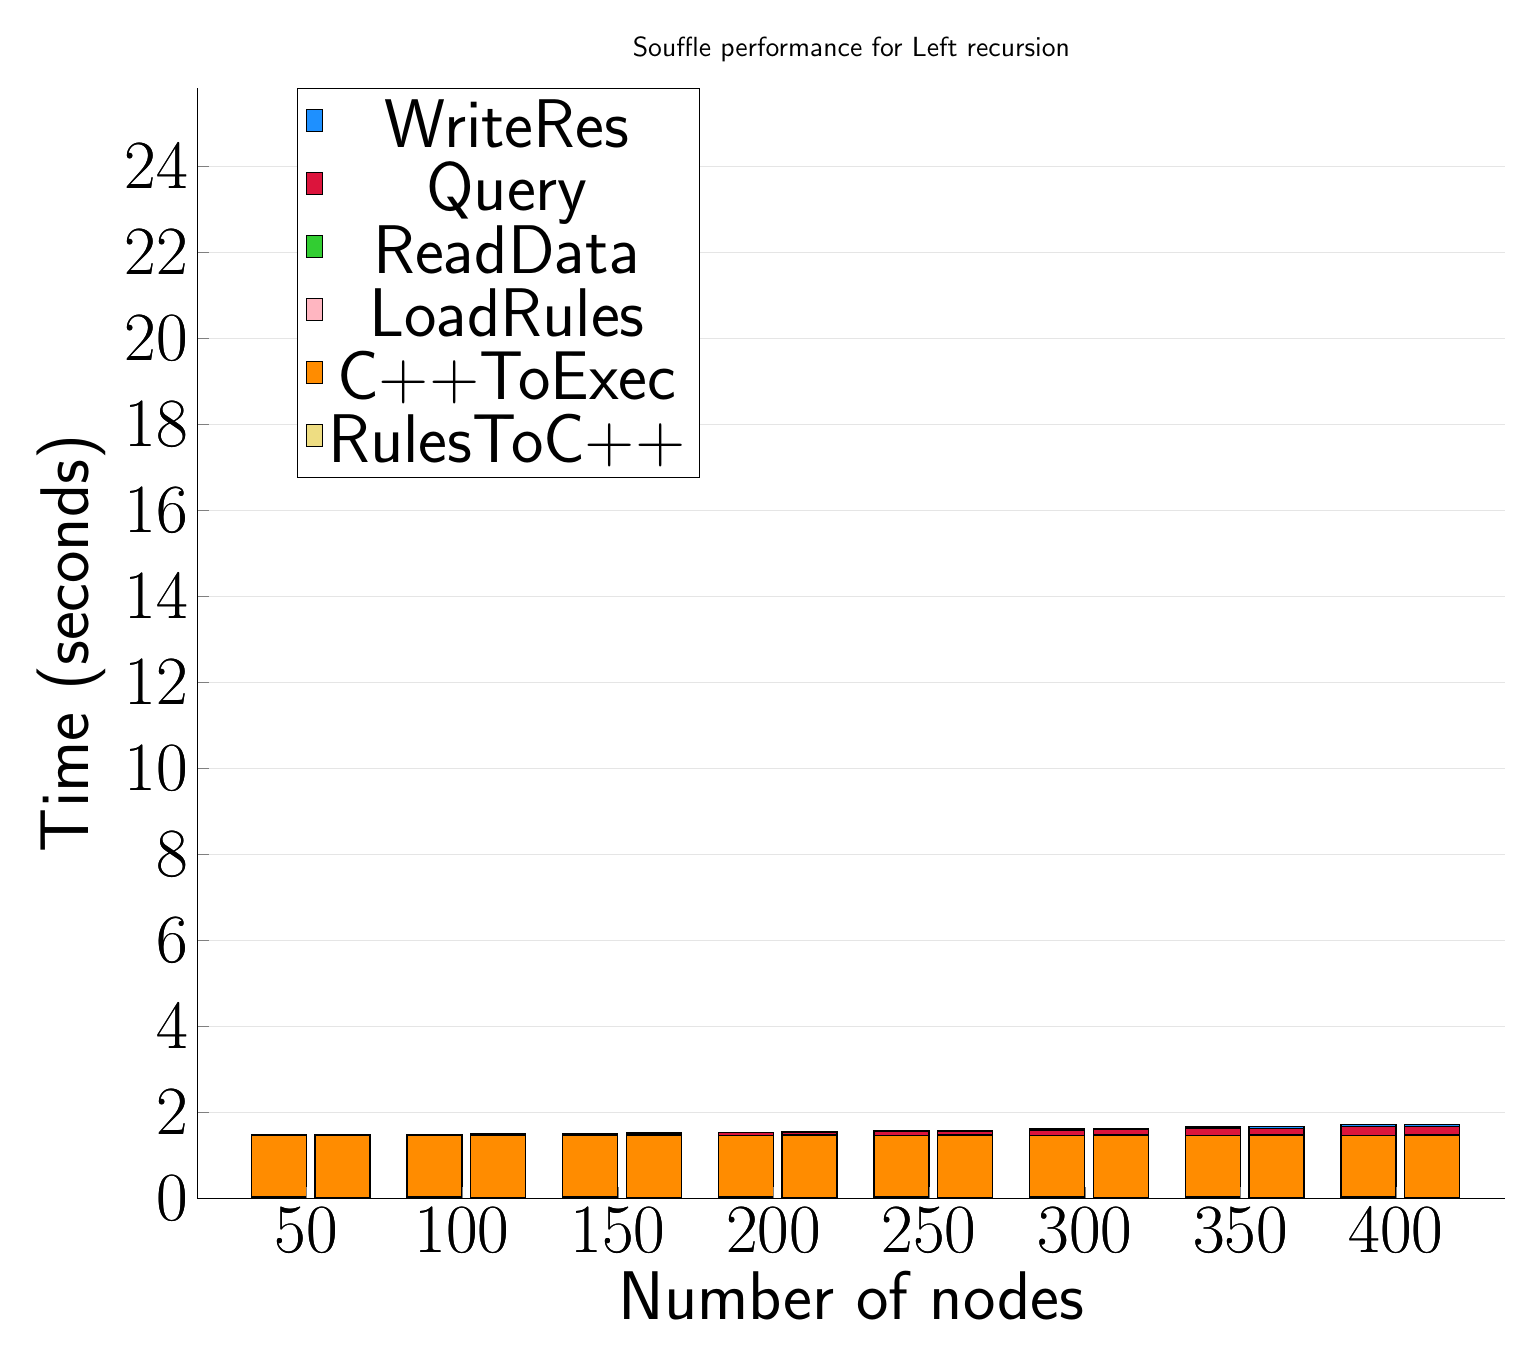
\begin{tikzpicture}
\begin{axis}[
   ybar stacked,
   title={Souffle performance for Left recursion},
   bar shift=-10pt,
   width=1.5\textwidth,
   bar width=0.7cm,
   ymajorgrids, tick align=inside,
   major grid style={draw=gray!20},
   xtick=data,
   ymin=0, ymax=25.820519999999995,
   axis x line*=bottom,
   axis y line*=left,
   enlarge x limits=0.1,
   legend style={
       at={(0.23, 1)},
       anchor=north,
       legend columns=1,
       font=\Huge,
   },
   ylabel={Time (seconds)},
   xlabel={Number of nodes},
   label style={font=\Huge},
   tick label style={font=\Huge},
]
\addlegendimage{fill=DodgerBlue, draw=black, line width=0.2pt}
\addlegendentry{WriteRes}
\addlegendimage{fill=Crimson, draw=black, line width=0.2pt}
\addlegendentry{Query}
\addlegendimage{fill=LimeGreen, draw=black, line width=0.2pt}
\addlegendentry{ReadData}
\addlegendimage{fill=LightPink, draw=black, line width=0.2pt}
\addlegendentry{LoadRules}
\addlegendimage{fill=DarkOrange, draw=black, line width=0.2pt}
\addlegendentry{C++ToExec}
\addlegendimage{fill=LightGoldenrod, draw=black, line width=0.2pt}
\addlegendentry{RulesToC++}
\addplot +[fill=LightGoldenrod, draw=black, line width=0.5pt] coordinates {
    (50, 0.039999961853027344)
    (100, 0.04000003337860107)
    (150, 0.04100000858306885)
    (200, 0.039999961853027344)
    (250, 0.039999985694885255)
    (300, 0.03900003433227539)
    (350, 0.04000000953674317)
    (400, 0.04000003337860107)
};
\addplot +[fill=DarkOrange, draw=black, line width=0.5pt] coordinates {
    (50, 1.4310000658035278)
    (100, 1.4230000019073485)
    (150, 1.4259999990463257)
    (200, 1.4320000171661378)
    (250, 1.4269999980926513)
    (300, 1.4299999952316285)
    (350, 1.4290000200271606)
    (400, 1.4239999771118164)
};
\addplot +[fill=LightPink, draw=black, line width=0.5pt] coordinates {
    (50, 7.54251e-05)
    (100, 9.91958e-05)
    (150, 0.00011410850000000001)
    (200, 0.0001102291)
    (250, 8.41041e-05)
    (300, 0.0001267668)
    (350, 0.0001227459)
    (400, 0.00012528340000000001)
};
\addplot +[fill=LimeGreen, draw=black, line width=0.5pt] coordinates {
    (50, 0.00030883340000000003)
    (100, 0.00044948340000000006)
    (150, 0.0006135916)
    (200, 0.0006669167)
    (250, 0.0007789584)
    (300, 0.0009259914999999999)
    (350, 0.0010063249)
    (400, 0.001143068)
};
\addplot +[fill=Crimson, draw=black, line width=0.5pt] coordinates {
    (50, 0.004033355)
    (100, 0.015665489999999997)
    (150, 0.03497678)
    (200, 0.0573419)
    (250, 0.08471237999999999)
    (300, 0.1181055)
    (350, 0.1580305)
    (400, 0.2055177)
};
\addplot +[fill=DodgerBlue, draw=black, line width=0.5pt] coordinates {
    (50, 0.00135905)
    (100, 0.003903945)
    (150, 0.008024270000000002)
    (200, 0.01170375)
    (250, 0.017732710000000002)
    (300, 0.025409019999999997)
    (350, 0.034545000000000006)
    (400, 0.04563025)
};
\end{axis}
\begin{axis}[
   ybar stacked,
   bar shift=13pt,
   width=1.5\textwidth,
   bar width=0.7cm,
   ymajorgrids, tick align=inside,
   major grid style={draw=none},
   xtick=data,
   ymin=0, ymax=25.820519999999995,
   axis x line*=none,
   axis y line*=none,
   enlarge x limits=0.1,
   label style={font=\Huge},
   tick label style={font=\Huge},
]
\addplot +[fill=LightGoldenrod, draw=black, line width=0.5pt] coordinates {
    (50, 0.031999999999999994)
    (100, 0.030000000000000006)
    (150, 0.030000000000000006)
    (200, 0.030000000000000006)
    (250, 0.030000000000000006)
    (300, 0.030000000000000006)
    (350, 0.030000000000000006)
    (400, 0.030000000000000006)
};
\addplot +[fill=DarkOrange, draw=black, line width=0.5pt] coordinates {
    (50, 1.448)
    (100, 1.4469999999999996)
    (150, 1.4469999999999998)
    (200, 1.452)
    (250, 1.448)
    (300, 1.4509999999999998)
    (350, 1.446)
    (400, 1.4459999999999997)
};
\addplot +[fill=LightPink, draw=black, line width=0.5pt] coordinates {
    (50, 7.48e-05)
    (100, 9.85e-05)
    (150, 0.0001135)
    (200, 0.00010960000000000002)
    (250, 8.34e-05)
    (300, 0.00012580000000000002)
    (350, 0.0001218)
    (400, 0.0001245)
};
\addplot +[fill=LimeGreen, draw=black, line width=0.5pt] coordinates {
    (50, 0.00030810000000000006)
    (100, 0.0004485)
    (150, 0.0006096)
    (200, 0.0006659000000000001)
    (250, 0.0007781)
    (300, 0.0009249999999999999)
    (350, 0.0010059000000000001)
    (400, 0.0011401000000000002)
};
\addplot +[fill=Crimson, draw=black, line width=0.5pt] coordinates {
    (50, 0.0040327)
    (100, 0.0156366)
    (150, 0.034923600000000006)
    (200, 0.057228)
    (250, 0.08456549999999999)
    (300, 0.1179374)
    (350, 0.15773580000000004)
    (400, 0.20520049999999998)
};
\addplot +[fill=DodgerBlue, draw=black, line width=0.5pt] coordinates {
    (50, 0.0013583)
    (100, 0.0038955000000000005)
    (150, 0.007509399999999999)
    (200, 0.0114633)
    (250, 0.017619199999999998)
    (300, 0.025294900000000002)
    (350, 0.0344206)
    (400, 0.0450318)
};
\end{axis}
\end{tikzpicture}

\end{document}
